\subsection{Task 3.1 -- Phương pháp và quyết định kiến trúc}

Nhóm mô tả BrewLite theo C4 ở ba mức gồm ngữ cảnh, container và thành phần API.
Web Next.js phục vụ giao diện mobile-first trên Vercel và chuyển tiếp yêu cầu
\nolinkurl{/api} sang NestJS trên Render. PostgreSQL chạy trên Supabase ở
production và trong Docker Compose ở local. Prisma quản lý schema và migration.

\begin{center}
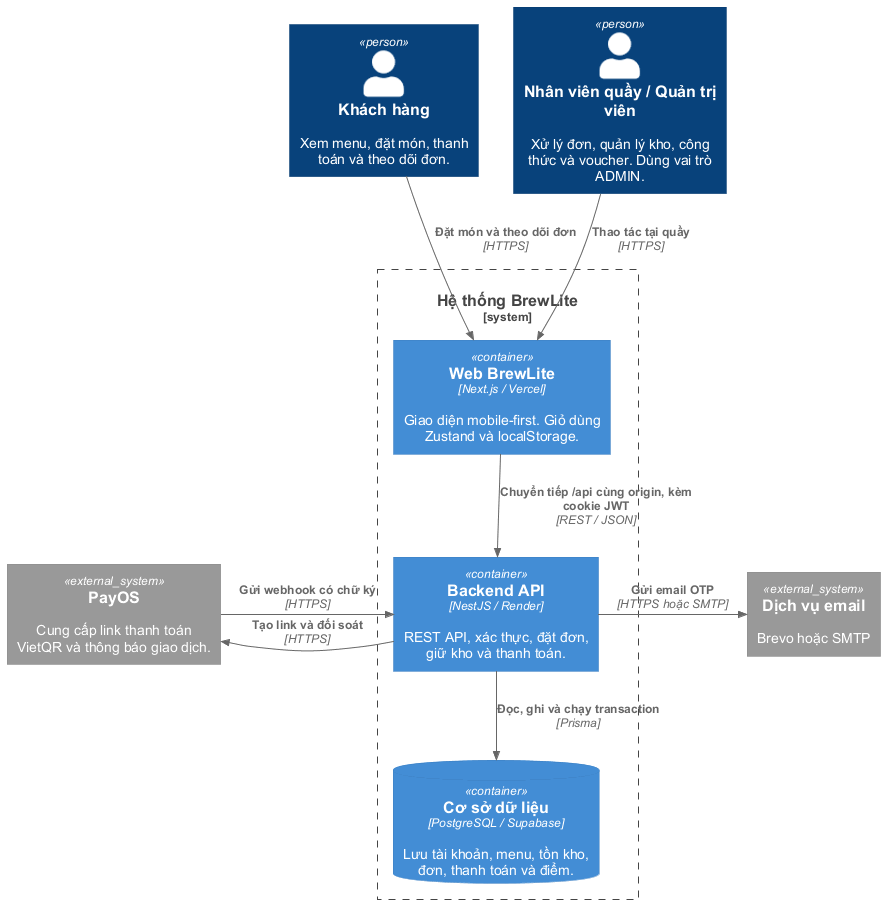
\includegraphics[width=\linewidth,height=0.69\textheight,keepaspectratio]{../../architecture/c4/c4-context-container.png}\\[0.5em]
{\small\itshape Hình 3.1a. Ngữ cảnh và các container của BrewLite (C4 mức 1 và 2)}
\end{center}

Tài liệu \nolinkurl{system-architecture.md} và sáu ADR trong
\nolinkurl{docs/architecture/} giải thích các luồng xử lý, cấu hình theo môi trường
và đánh đổi kiến trúc. Mã nguồn sơ đồ nằm trong \nolinkurl{docs/architecture/c4/}.

\clearpage
\subsubsection*{Thành phần API và các quyết định kiến trúc}
NestJS chạy dưới dạng modular monolith. Cách này giúp tạo đơn, giữ kho theo
công thức và xác nhận thanh toán bằng transaction PostgreSQL. Các module chia
sẻ tài nguyên của một tiến trình API. Checkout xử lý thẻ mô phỏng nội bộ và
dùng PayOS cho VietQR. API xác thực JWT, kiểm tra quyền, ghi log bằng NestJS
và kiểm tra PostgreSQL qua \nolinkurl{/api/health}.

\begin{center}
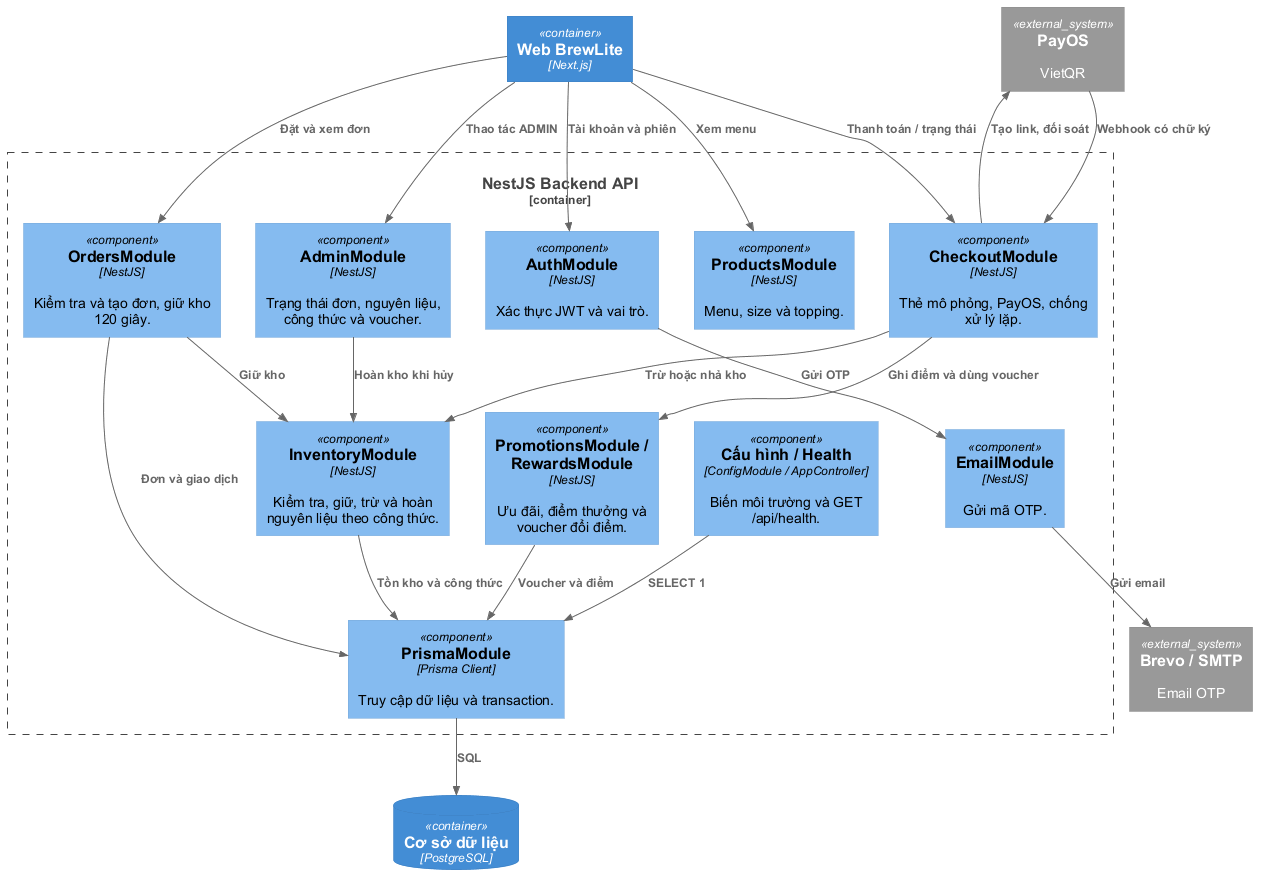
\includegraphics[width=\linewidth,keepaspectratio]{../../architecture/c4/c4-backend-components.png}\\[0.5em]
{\small\itshape Hình 3.1b. Các thành phần chính của NestJS API (C4 mức 3)}
\end{center}
